\documentclass[10pt]{article}
\usepackage[margin=1in]{geometry}
\usepackage{amsmath,amssymb,graphicx,booktabs,hyperref,natbib}
\hypersetup{hidelinks}
\title{Selection of Feature-Sparse Ensembles: Co-Error, Certification, and Generalization}
\author{Research draft}
\date{Living development manuscript; not a submission-ready evaluation}
\begin{document}
\maketitle
\begin{abstract}
We investigate ensembles selected from large populations of feature-sparse weak
predictors. The study asks whether empirical skill screening and explicit error
complementarity improve generalization beyond random subspaces and ordinary
validation-based ensemble selection. Squared-error and binary Brier losses admit
an exact residual second-moment objective, whereas correlation-based diversity
discards scale and can penalize useful negative dependence. The protocol reserves
outer test folds, compares methods on shared candidate populations, and records
selection and computational costs. An initial synthetic study finds modest gains
over quality selection, severe screening infeasibility, and false survivors under
the null, while strong forest and boosting baselines generally perform better.
An oracle additive counterexample identifies attenuation from averaging subspaces,
motivating an affine-profiled diagnostic. Results remain development evidence;
no benchmark superiority or novelty claim is established.
\end{abstract}
\section{Introduction}
Useful tabular information may be distributed across weakly informative subspaces.
Selecting complementary errors could improve an average of weak predictors, but
this hypothesis competes with simpler explanations: regularization, more search
compute, and ordinary ensemble selection. We test these alternatives using paired
candidate pools and known synthetic mechanisms. Sparse signal and interactions
provide explicit potential counterexamples.


\section{Related Work and Unresolved Novelty}
Bagging \citep{breiman1996} and random forests \citep{breiman2001} reduce instability
through aggregation. Random subspaces \citep{ho1998} assign fixed feature subsets
to trees; random patches \citep{louppe2012} also sample rows. RaSE
\citep{tian2021} already generates and selects random subspaces, making a claim
to novelty based on subspace search alone untenable. Ensemble selection
\citep{caruana2004} optimizes validation ensemble performance from a model library.
The ambiguity decomposition \citep{krogh1995} motivates squared-loss aggregation;
diversity can help or hurt majority votes \citep{brown2010}. These precedents
require differentiating any eventual contribution through mechanism, statistical
procedure, scaling, or a substantiated algorithmic improvement.
Stacking, negative correlation learning, pruning, portfolio objectives, and
random projections require further primary-source review before submission.


\section{Method}
Candidate $b$ has a fixed raw-feature mask $F_b$, tree depth, leaf-size constraint,
row-sampling fraction, and seed, specified before fitting. Fold-local preprocessing
and the tree see only $F_b$. Inner cross-fitting yields predictions $P_{nb}$.
Binary screening uses a stratified empirical bootstrap lower AUROC quantile;
regression uses cross-fitted null-relative squared-error skill. We retain this as
a heuristic screen, not a familywise certificate.

\subsection{Theoretical Motivation}
Let $E_{nb}=y_n-P_{nb}$ and $G=E^\top E/N$. For an equal-weight subset $S$ of
cardinality $K$,
\begin{equation}
\widehat L_{\mathrm{sq}}(S)=K^{-2}\sum_{i,j\in S}G_{ij}.
\end{equation}
This is an algebraic identity for regression MSE and binary Brier loss, not a
generalization bound. Writing $\mu=N^{-1}E^\top\mathbf 1$ gives
$G=C+\mu\mu^\top$. Correlation removes marginal scale and mean; covariance
alone removes bias. Neither equals squared ensemble loss. Statistical independence
does not follow from zero correlation. Prediction correlation, error correlation,
and useful ensemble complementarity are distinct.

For multiclass probabilities, define vector residuals $r_{ni}=u_{y_n}-p_{ni}$,
where $u_y$ is one-hot. We use $G_{ij}=N^{-1}\sum_n r_{ni}^\top r_{nj}$,
giving sum-over-classes Brier loss. Classwise means $\mu_{ic}$ yield
$G_{ij}=\sum_c C_{ij,c}+\sum_c\mu_{ic}\mu_{jc}$; covariance-only and
shrinkage preserve this distinction. The initial multiclass correlation selectors
apply Pearson correlation to flattened sample/class residual coordinates.
Because each probability vector sums to one, the flattened residual means are
zero and this correlation is $G_{ij}/\sqrt{G_{ii}G_{jj}}$. It retains classwise
bias and should not be interpreted as a correlation of class-centered residuals.
This convention is recorded explicitly before interpreting the wine results.

We compare random selection, empirical quality, absolute and signed error
correlation, minimax dependence, quality--dependence tradeoffs, and greedy
co-error followed by improving one-swaps. Direct squared-loss selection without
replacement is exactly the same greedy objective, so it supplies a verification
baseline rather than a separate contribution. A with-replacement Caruana-style
baseline yields nonuniform weights and is labeled separately.

\subsection{Bias-Preserving Shrinkage Variant}
We additionally test $G_\alpha=(1-\alpha)C+\alpha\operatorname{diag}(C)+\mu\mu^\top$.
Shrinkage could reduce noisy cross-moment exploitation as the pool grows. It can
also suppress genuine complementarity. The falsifying experiment holds $K$ fixed,
varies $B/N$, and measures outer loss and selection optimism. This regularizer
has no established novelty or superiority claim.

\subsection{An Oracle Attenuation Counterexample}
Suppose $Y=\sum_{j=1}^d s_j(X_j)+\epsilon$, with independent centered signal
components of equal variance $v$, independent centered noise of variance
$\sigma^2$, and population-optimal subspace learners
$f_b=\mathbb E[Y\mid X_{F_b}]=\sum_{j\in F_b}s_j(X_j)$.
Define $w_j=K^{-1}\sum_{b\in S}\mathbb I(j\in F_b)$. Then
\begin{equation}
L(S)=\sigma^2+v\sum_{j=1}^d(1-w_j)^2.
\end{equation}
If each mask contains at most $q<d$ informative features, then
$\sum_j w_j\le q$ and Jensen's inequality yields
$L(S)\ge\sigma^2+dv(1-q/d)^2$. Thus averaging individually optimal subspace
predictors attenuates distributed additive signal, even when their union covers
all informative coordinates and $B,K$ are arbitrarily large. For the additive
regression development design, $d=16$, $v=1/16$, $q\le4$, and $\sigma^2=1$,
so this idealized conditional-mean ensemble has risk at least $1.5625$.
This is a population calculation for these oracle learners, not a lower bound
for arbitrary subspace functions, finite-sample fitted trees, or classification
AUROC. Coordinated fitting or non-simplex rescaling can escape its assumptions.
It motivates testing aggregate scale calibration separately from diversity.

\subsection{Affine-Profiled Diagnostic Variant (APCE)}
After Experiment 001, we test an affine correction $a\bar P_S+b$, with $a\ge0$
and intercept $b$ fitted exclusively on training OOF predictions. For a fixed
subset, the profiled squared loss is
\begin{equation}
\widehat L_{\mathrm{aff}}(S)=\widehat{\operatorname{Var}}(Y)
-\frac{\max(\widehat{\operatorname{Cov}}(Y,\bar P_S),0)^2}
{\widehat{\operatorname{Var}}(\bar P_S)}.
\end{equation}
Zero aggregate variance gives the constant predictor. Centered prediction moments
support incremental greedy and one-swap updates. The comparison includes affine
correction of unchanged random, top-quality, and co-error subsets, isolating
selection from the two new aggregation parameters. This is a stacking-like
diagnostic and is not claimed as a novel optimizer or equal-output-weight primary method.

\section{Experimental Protocol}
All initial settings are fixed before each run. Outer folds remain unused during
candidate screening and selection; selected specifications are refitted on the
full outer training fold. Any future tuning regenerates the complete pipeline
inside an additional tuning split, rather than slicing a globally fitted OOF
matrix. All baselines share outer splits and fold-local preprocessing.
Development synthetic regimes are separate from any locked real-world confirmation
suite. Binary AUROC and regression RMSE are primary; multiclass log loss is primary.
Brier loss is additionally central to the mechanism analysis. Bootstrap intervals
over fixed OOF rows omit training instability, and unadjusted candidate screens
omit multiplicity. These limitations prohibit interpreting them as simultaneous
statistical certification.
Shared candidate-search cost is charged to every standalone selector. Capacity
and inference measurements accompany accuracy; matched-budget claims require
dedicated experiments. Paired task-level analyses average folds and seeds before
resampling tasks. No row-level significance claims across tasks are permitted.


\section{Synthetic Experiments}
% Generated from frozen experiment artifacts; do not edit.
\newcommand{\ExpOneOuterFolds}{108}
\newcommand{\ExpOneBinaryFeasible}{40}
\newcommand{\ExpOneRegressionFeasible}{16}
\newcommand{\ExpOneNullMin}{3}
\newcommand{\ExpOneNullMax}{13}
\newcommand{\ExpOneAdditiveCoerror}{0.899}
\newcommand{\ExpOneAdditiveForest}{0.784}
\newcommand{\ExpOneAdditiveCatboost}{0.764}
\newcommand{\ExpOneAucGain}{0.0107}

Experiment 001 evaluated nine known mechanisms for each of binary classification
and regression: additive, redundant, correlated blocks, sparse, dominant, XOR,
four-way parity, mixed, and null. Fixed settings were $N=600$, $M=40$, $B=100$,
$K=8$, feature fraction $0.1$, tree depth 3, minimum leaf size 5, two generation
seeds, three outer folds, and three OOF folds. This produced
\ExpOneOuterFolds{} paired outer evaluations. Forest and boosting baselines use
static configurations; search compute, final capacity, and inference budgets
are measured but unmatched.

\begin{table}[t]
\centering\small
\begin{tabular}{lrrrrrrr}
\toprule
Regime & RS & Top & AbsCorr & CoErr & CoErr-all & RF & CatBoost \\
\midrule
additive & 0.655 & 0.689 & 0.701 & 0.693 & 0.693 & 0.809 & 0.794 \\
correlated\_blocks & 0.805 & 0.775 & 0.822 & 0.804 & 0.804 & 0.842 & 0.849 \\
dominant & 0.752 & 0.875$^{\dagger}$ & 0.867$^{\dagger}$ & 0.872$^{\dagger}$ & 0.872 & 0.869 & 0.886 \\
mixed & 0.588 & 0.662 & 0.672 & 0.666 & 0.666 & 0.705 & 0.746 \\
null & 0.506 & 0.527$^{\dagger}$ & 0.535$^{\dagger}$ & 0.509$^{\dagger}$ & 0.529 & 0.500 & 0.522 \\
parity & 0.528 & -- & -- & -- & 0.503 & 0.502 & 0.500 \\
redundant & 0.826 & 0.805 & 0.840 & 0.827 & 0.827 & 0.868 & 0.872 \\
sparse & 0.645 & 0.778 & 0.820 & 0.815 & 0.815 & 0.849 & 0.868 \\
xor & 0.483 & 0.478$^{\dagger}$ & 0.481$^{\dagger}$ & 0.494$^{\dagger}$ & 0.495 & 0.605 & 0.838 \\
\bottomrule
\end{tabular}
\caption{exp\_001\_mechanisms\_v1: binary, auroc. Means over completed outer folds and seeds. --: fixed-K infeasible in every split; $\dagger$: partial feasibility. Full coverage is stored separately. Static baselines, unmatched compute; development only.}
\end{table}

\begin{table}[t]
\centering\small
\begin{tabular}{lrrrrrrr}
\toprule
Regime & RS & Top & AbsCorr & CoErr & CoErr-all & RF & CatBoost \\
\midrule
additive & 0.933 & -- & -- & -- & 0.899 & 0.784 & 0.764 \\
correlated\_blocks & 0.735 & 0.750$^{\dagger}$ & 0.713$^{\dagger}$ & 0.723$^{\dagger}$ & 0.718 & 0.615 & 0.606 \\
dominant & 0.890 & 0.525$^{\dagger}$ & 0.525$^{\dagger}$ & 0.523$^{\dagger}$ & 0.515 & 0.511 & 0.514 \\
mixed & 0.974 & -- & -- & -- & 0.904 & 0.846 & 0.814 \\
null & 1.007 & -- & -- & -- & 1.018 & 1.038 & 1.018 \\
parity & 1.009 & -- & -- & -- & 1.027 & 1.039 & 1.023 \\
redundant & 0.691 & 0.701 & 0.686 & 0.687 & 0.687 & 0.591 & 0.580 \\
sparse & 0.925 & 0.797$^{\dagger}$ & 0.795$^{\dagger}$ & 0.797$^{\dagger}$ & 0.744 & 0.639 & 0.617 \\
xor & 1.021 & -- & -- & -- & 0.987 & 0.978 & 0.852 \\
\bottomrule
\end{tabular}
\caption{exp\_001\_mechanisms\_v1: regression, normalized\_squared\_loss. Means over completed outer folds and seeds. --: fixed-K infeasible in every split; $\dagger$: partial feasibility. Full coverage is stored separately. Static baselines, unmatched compute; development only.}
\end{table}

\begin{figure}[p]
\centering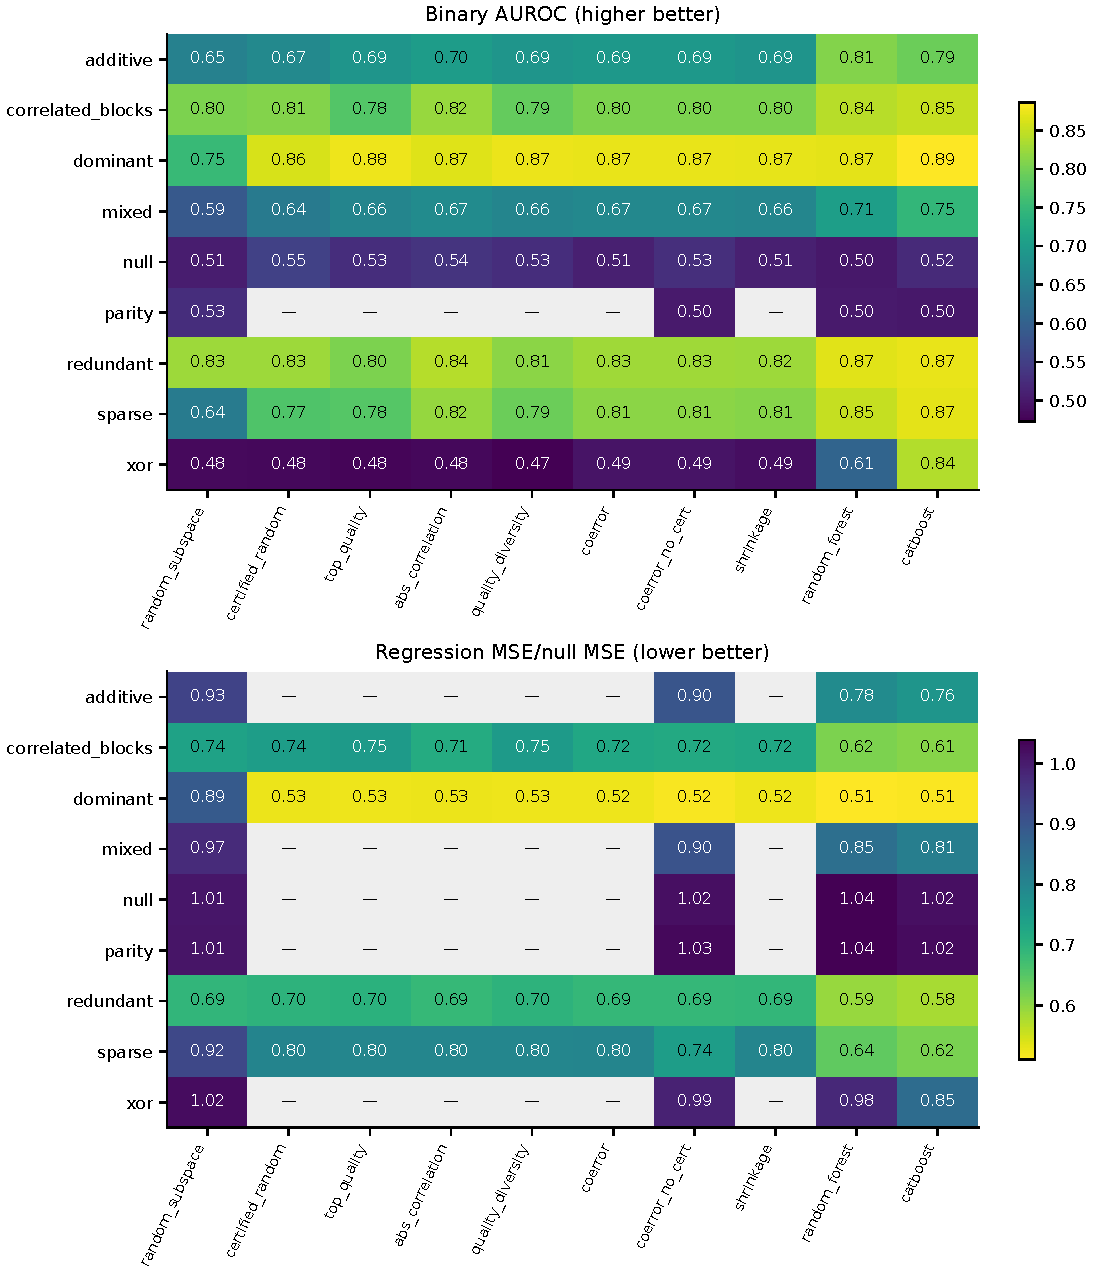
\includegraphics[width=\linewidth]{figures/exp_001_mechanisms_v1/performance.pdf}
\caption{Development mechanism results. Gray cells indicate no feasible fixed-$K$
screened ensemble. Numerical annotations are means of completed splits; the
tables mark partial feasibility. Rankings are not confirmation evidence.}
\end{figure}

The initial hypothesis is not supported as a broad performance claim at these
settings. Unfiltered co-error improves mean binary AUROC over unfiltered top
quality by \ExpOneAucGain{}, but generally trails the strong forests and boosting
models. Co-error does not consistently improve over absolute residual correlation
on outer AUROC or squared loss; a positive aggregate Brier effect is concentrated
in the dominant-feature regime. The $\alpha=0.5$ shrinkage variant fails to improve
on unregularized co-error in the compared task means. These are negative findings
for the preregistered settings, not universal statements about the objectives.

\subsection{Screening Failure and Feasibility}
Screened co-error is feasible in only \ExpOneBinaryFeasible{} of 54 binary splits
and \ExpOneRegressionFeasible{} of 54 regression splits. On every binary null
split, \ExpOneNullMin{}--\ExpOneNullMax{} of 100 candidates pass the empirical
screen, despite population AUROC $0.5$ under this data-generating process.
The bootstrap lower quantile must therefore remain labeled an empirical screen.
Across shared feasible splits, top-quality screening has almost no incremental
benefit over unscreened top quality; it frequently prevents a fixed-size ensemble.

\begin{figure}[t]
\centering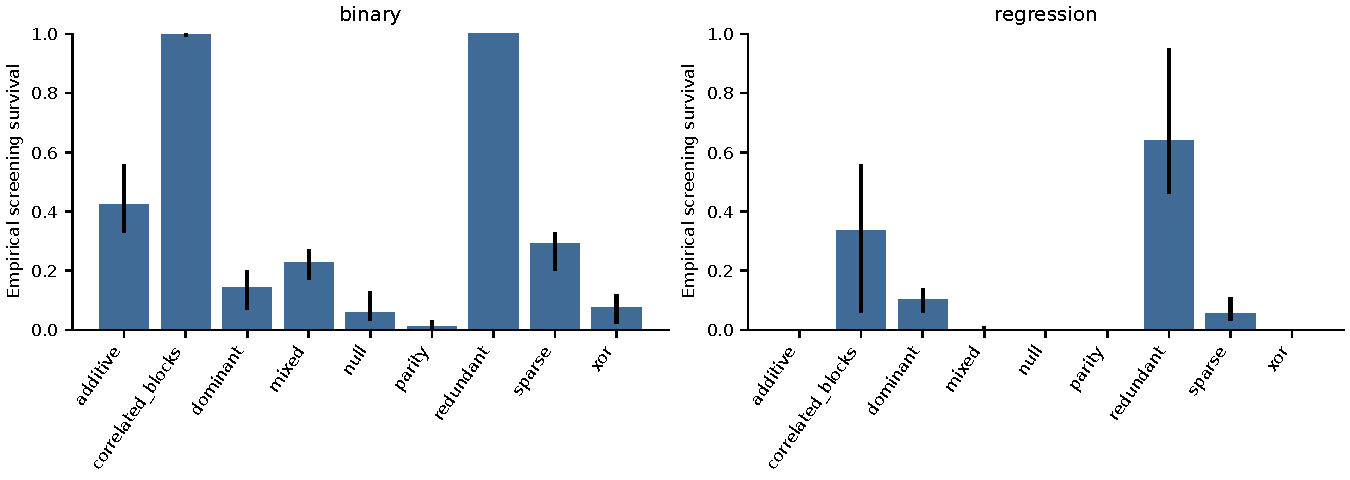
\includegraphics[width=\linewidth]{figures/exp_001_mechanisms_v1/certification.pdf}
\caption{Empirical screening survival by regime. Error bars give the observed
minimum and maximum over folds/seeds, not confidence intervals.}
\end{figure}

\section{Real-World Benchmarks}
No confirmation benchmark has been evaluated. Current benchmark versions and
baseline requirements will be recorded before locking the study.

\section{Ablations and Analysis}
The stored ablations include all required v0 components, signed versus absolute
residual correlation, prediction correlation, covariance without bias, direct
squared-loss greedy selection, with-replacement selection, and shrinkage. An
artifact audit reconstructed loss and test metrics for all selected methods;
the maximum squared-loss/co-error identity discrepancy was below $10^{-12}$.
Direct squared-loss and co-error greedy validation objectives agree, confirming
that their distinction supplies no additional mechanism.

\section{Analysis and Next Discriminating Test}
Additive regression illustrates the attenuation concern: normalized squared loss
is \ExpOneAdditiveCoerror{} for unfiltered co-error, versus
\ExpOneAdditiveForest{} for the unrestricted forest and
\ExpOneAdditiveCatboost{} for CatBoost. This observation does not establish that
attenuation is the sole cause. The next development experiment will compare
the same selected subsets with and without an OOF-fitted aggregate affine
calibrator, then test selection with the affine loss profiled out. Random and
top-quality controls are necessary to determine whether a change comes from
aggregate calibration or a new selection mechanism. Null and dominant-feature
controls will test increased selection/aggregation overfitting.

\section{Limitations}
This draft does not establish a novel algorithm or strong benchmark performance.
OOF selection risks overfitting to a reused training prediction matrix. Refitting
changes the fitted functions and may change their error dependence. IID row
bootstrap screens do not justify guarantees under overlapping training folds,
large candidate libraries, grouped observations, or temporal shifts. Sparse
shallow trees can fail on interactions that need joint feature access.

\section{Conclusion}
The research program tests whether feature-sparse error complementarity supplies
an advantage beyond established subspace and ensemble-selection methods. Conclusions
will follow stored paired experiments, including negative results.


\bibliographystyle{plainnat}
\bibliography{bibliography}
\end{document}
